\section{Porous Media}
\subsection{Author and source}
The porous media test-case is derived from the paper \cite{Aarnes_2007}. A copy of the source code is included in the \texttt{git} repository, with some minor modifications to run the 3D version of the model, as described below. The application is a finite volume code that simulates a toy model of a reservoir.
\subsection{Description of the mathematical formulation}\label{power_cont_adj_math}
Detailed mathematical formulation is given in \cite{Aarnes_2007}
\subsection{Directory structure and description of files}
The porous media test-case is organized into following directories and subdirectories:\\

\dirtree{%
.1 /. 
.2 MATLAB\DTcomment{Original files with some modifications for 3D}.
.3 MATLAB/data\DTcomment{Data about the reservoir}.
.3 MATLAB/2phase\DTcomment{Saturation solver and drivers for 2-phase simulator}.
.3 MATLAB/TPFA\DTcomment{Two-point flux approximation method}. 
.3 MATLAB/MFEM\DTcomment{Mixed finite element method}. 
.2 Fortran\DTcomment{Fortran version of porous media model}. 
.3 Fortran/Port\DTcomment{Port of the \texttt{MATLAB} version}. 
.3 Fortran/DiscreteAdj/OpenAD/joint\DTcomment{Incomplete OAD version}. 
}
\hfill\break
\noindent Some of the descriptions for the \texttt{MATLAB} directories were obtained from the \texttt{README} file that comes with the original code.
\clearpage
\subsubsection{\texttt{MATLAB} version}
The directory \texttt{MATLAB} contains the original files with some minor changes to run the 3D version of the porous media model.\\

\noindent The listing of files and their descriptions follow.\\
\dirtree{%
.1 /. 
.2 data. 
.3 spe10.mat\DTcomment{Porosity and Permeability data}. 
.2 2phase. 
.3 GenA.m\DTcomment{Matrix with upwind FV stencil}. 
.3 runq5.m\DTcomment{Simulator for homogeneous quarter-five spot}. 
.3 runspe10.m\DTcomment{Simulator for the top layer of SPE-10 model}. 
.3 RelPerm.m\DTcomment{Relative permeabilities of oil and water}. 
.3 Pres.m\DTcomment{Pressure solver}. 
.3 Upstream.m\DTcomment{Explicit upwind finite-volume discretization}. 
.3 NewtRaph.m\DTcomment{Implicit upwind finite-volume discretization}. 
.3 runspe10wplot.m\DTcomment{Ditto \texttt{runspe10.m} with plot}. 
.2 TPFA. 
.3 TPFA.m\DTcomment{Two-point flux approximation scheme}. 
.3 run.m\DTcomment{Driver to test \texttt{TPFA.m}}. 
.2 README\DTcomment{Directory map, howtos,  disclaimer}. 
.2 MFEM\DTcomment{Unused currently}. 
.3 GenB.m. 
.3 plotsl.m. 
.3 runSPE10.m. 
.3 GenC.m. 
}
\hfill\break
\noindent The \texttt{MATLAB} version can be executed like below.\\

\begin{lstlisting}[language=mymatlab, numbers=none]
>> cd 2phase
>> addpath('../TPFA/')
>> runspe10wplot
\end{lstlisting}
\hfill \break
\noindent The plots generated by the \texttt{MATLAB} version appear on the following page.
\begin{NotePar}
\noindent The \texttt{MATLAB} plots were obtained with setting the number of grid elements along \textit{x} and \textit{y} to be 32 and that along \textit{z} to be 1. The inflow was set to be the bottom-left corner and top-right corner for the outflow.
\end{NotePar}
\clearpage
\begin{figure}[h]
\centering
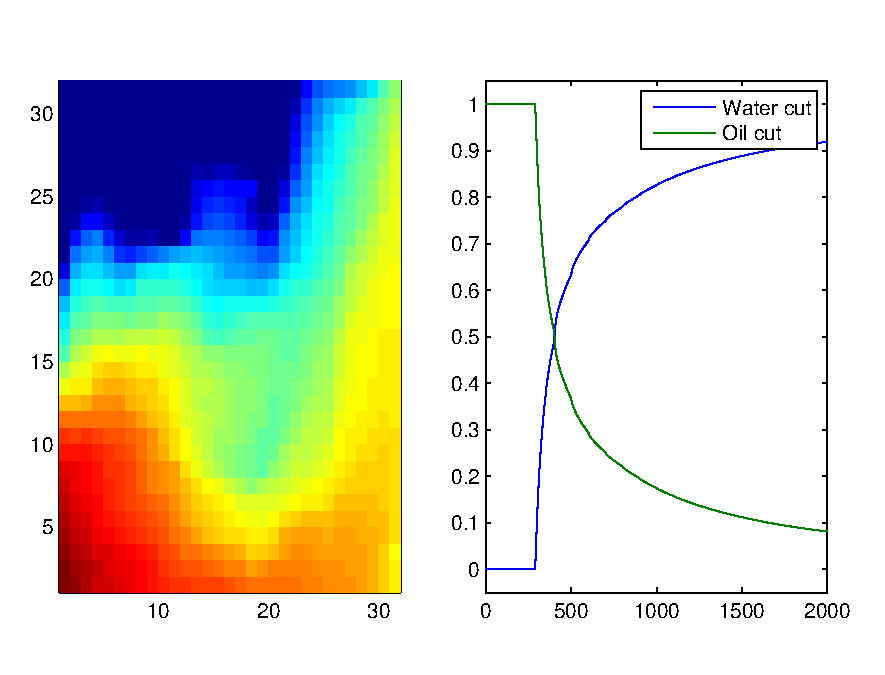
\includegraphics[width=1.2\linewidth]{../Code/miniApps/porous_media/matlab_pm.eps}
\caption{Plot of Saturation and Production curves from SPE10 model using MATLAB}
\label{fig:plot_of_saturation_production}
\end{figure}
\clearpage
\subsubsection{\texttt{Fortran} port}\label{sec_fortran_port_porous}
The directory \texttt{Fortran/Port} contains the port of the \texttt{MATLAB} version. MGMRES \cite{Barrett_1994},\cite{Kelley_1995} and \cite{Saad_2003} was used to solve the sparse linear system in the \texttt{Fortran} port, a copy of which can be obtained \href{http://people.sc.fsu.edu/~jburkardt/m_src/mgmres/mgmres.html}{here}.\\

\noindent The directory \texttt{Fortran/Port} contains the files to compile the two-phase, immiscible, incompressible simulator for the SPE-10 model using implicit upwind finite-volume discretization as listed in \cite{Aarnes_2007}. The binary (\textbf{file}), corresponding to this, on building the directory is \texttt{porous\_media} (\textbf{{runspe10.f90}}).\\

\noindent The listing of files and their descriptions follow.\\

\dirtree{%
.1 /. 
.2 Fortran/Port.  
.3 fluid.f90\DTcomment{Constants - viscosities and irreducible saturations}. 
.3 fvm.f90\DTcomment{Methods related to finite volume discretization}. 
.3 gnufor2.f90\DTcomment{Fortran bindings for GNUPlot}. 
.3 grid.f90\DTcomment{Constants - grid size, step size, cell volume}. 
.3 KUr.txt\DTcomment{Permeability data}. 
.3 linsolve.f90\DTcomment{Wrapper to linear solvers}. 
.3 Makefile\DTcomment{Build commands}. 
.3 mathutil.f90\DTcomment{Commonly used math utilities - norm}. 
.3 matrix.f90\DTcomment{Sparse matrix definition and operations}. 
.3 mgmres.f90\DTcomment{Restarted GMRES solver for sparse linear systems}. 
.3 print\_active.f\DTcomment{Routines to pretty print matrices and vectors}. 
.3 pUr.txt\DTcomment{Porosity data}. 
.3 runspe10.f90\DTcomment{Simulator for the top layer of SPE-10 model}. 
.3 spdiags\_matlabtest.m\DTcomment{Examples of \texttt{MATLAB spdiags}}. 
.3 test\_fortran\_wholearray\_ops.f90\DTcomment{\texttt{Fortran} whole array ops test}. 
.3 test\_implied\_do\_loop.f90\DTcomment{Implied do loop in \texttt{Fortran}}. 
.3 test\_linsolve.f90\DTcomment{Script to test \texttt{linsolve} module}. 
.3 test\_mat\_read.f90\DTcomment{Test reading \texttt{MATLAB} multi-dimensional arrays}. 
.3 test\_openad\_features.f90\DTcomment{Test reshape through \texttt{OpenAD/F}}. 
.3 test\_sparse\_matrix.f90\DTcomment{Test \texttt{Fortran} spdiags implementation}. 
.3 test\_tpfa.f90\DTcomment{Test two-point flux approximation routine}. 
}
\hfill \break
\noindent The plot of data generated by the \texttt{Fortran} port appears on the following page.
\begin{NotePar}
\noindent The data from \texttt{Fortran} port for plots were obtained by setting the number of grid elements along \textit{x} and \textit{y} to be 32 and that along \textit{z} to be 1. The inflow was set to be the bottom-left corner and top-right corner for the outflow.
\end{NotePar}
\clearpage
\begin{figure}[h]
\centering
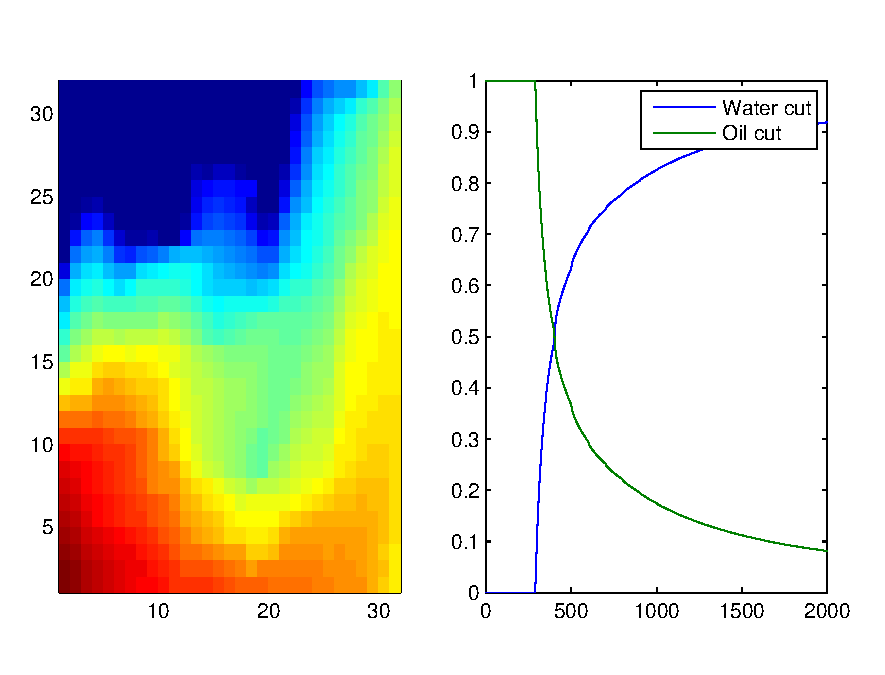
\includegraphics[width=1.2\linewidth]{../Code/miniApps/porous_media/fortran_pm.eps}
\caption{Plot of Saturation and Production curves from SPE10 model using FORTRAN port}
\label{fig:plot_of_saturation_production_for}
\end{figure}
\clearpage
\subsubsection{\texttt{Fortran} port with \texttt{OpenAD/F} in Reverse Joint Mode}
\begin{TodoPar}
\noindent The adjoint model of the \texttt{Fortran} port using \texttt{OpenAD/F} is still a work in progress. For now, the directory \texttt{Fortran/DiscreteAdj/OpenAD/joint} contains pretty much the same code as the \texttt{Fortran} port itself.
\end{TodoPar}
%\subsection{Modifications performed}
\subsection{How to build}
Running make as below, in the \texttt{Fortran/Port} subdirectory will build the  binary \texttt{porous\_media}
\hfill\break
\begin{lstlisting}[language=mybash, numbers=none]
    $ make
\end{lstlisting}
\subsection{How to verify}
At the time of writing, there exists no script that can validate the output from the \texttt{Fortran} port with that from the \texttt{MATLAB} version. \\

\noindent Validation by plotting the output from each version has been performed. 

\begin{TodoPar}
\noindent It will be valuable to follow the idea laid out in section \ref{airfoil_verify} and setup the infrastructure to validate the outputs from \texttt{Fortran} port with that from the \texttt{MATLAB} version.
\end{TodoPar}

%\subsection{How to extend}